\chapter{Deliverable methodology}
The KRUT-methodology (including the Swedish usability testing manuscript) created for this study is an inspirational tool for usability testing teaching materials. In true accessibility spirit, it is encouraged for users to make modifications to this as deemed appropriate and share the revised version with others. For easy access, this deliverable was included at the very end of this study report. 

\mbox{}
\begin{sidewaysfigure}
%\centering
\section{KRUT-methodolgy}
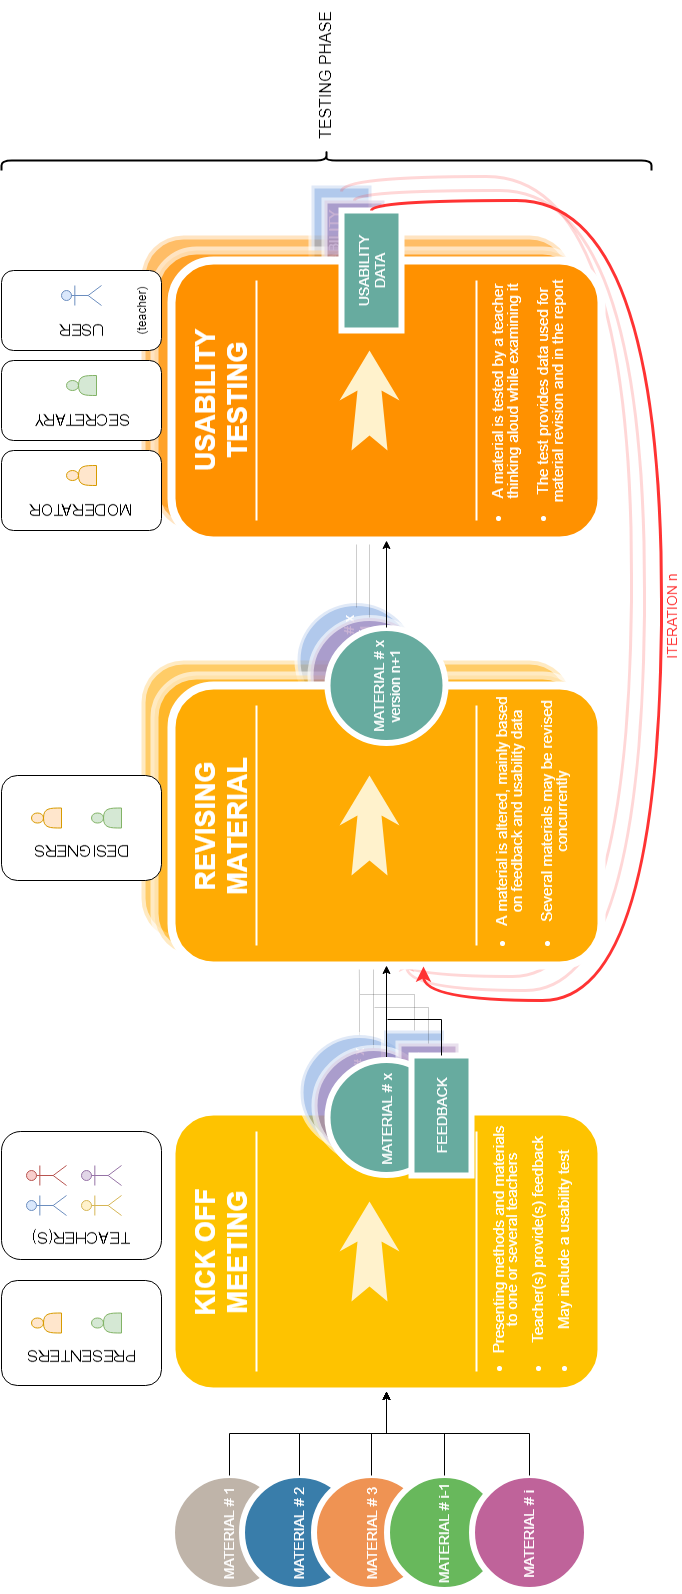
\includegraphics[trim={0 0cm 0 0},clip,width=0.4\textwidth,angle=-90]{figure/workflow.png}
\vspace*{2cm}
\caption{The custom KRUT-methodology, created for usability testing teaching materials.}
\label{app:krut}
\end{sidewaysfigure}

\newpage
\section{The KRUT usability testing manuscript}
In this study, a manuscript was created for usability testing the teaching materials. This manuscript is written in Swedish and can be used as a template for anyone interested. This manuscript was created with the assumption that the test subject is presented with a list of teaching materials, and would start the test by deciding what material is to be tested. As the situation probably will differ when other people test a material, it is encouraged that the manuscript is modified based on any current needs. It is also encouraged that any changes made to the manuscript and any findings made from usability testing teaching materials are shared publicly, so that as many as possible can benefit.

\begin{figure}[h]
\frame{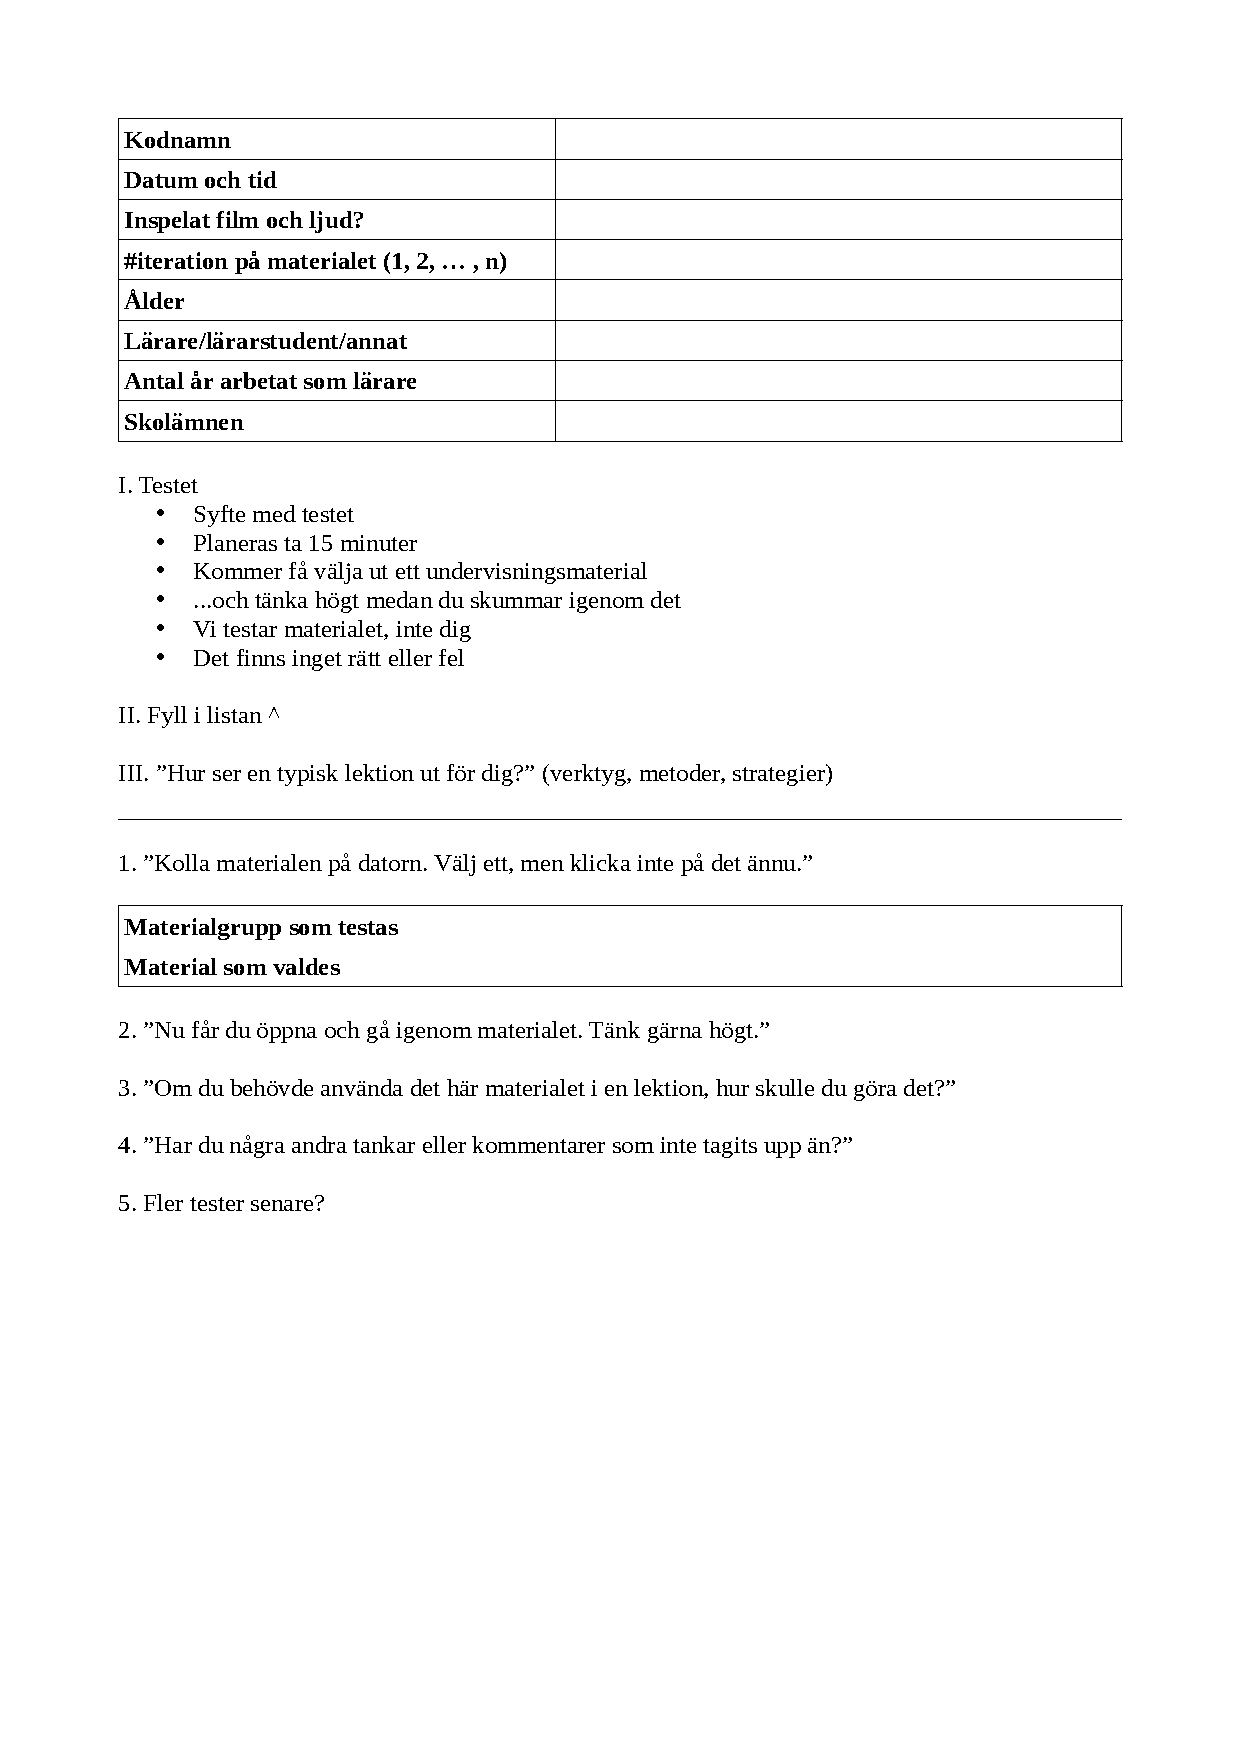
\includegraphics[trim={0 8cm 0 1cm},clip,page=1,width=0.8\textwidth]{pdf/template}}
\caption{The custom manuscript, used when usability testing teaching materials.}
\label{app:script}
\end{figure}

This manuscript can also be found as a editable text document on any of the following links:

\url{https://github.com/Niwsters/teaching-materials-thesis/raw/master/usability_tests/usabilitytest_mall.odt}

\url{https://goo.gl/vauvUR} (note that this url is case-sensitive).
